\documentclass[a4paper,14pt]{extarticle}

\usepackage[top=1in, bottom=1in, left=1in, right=1in]{geometry}
\usepackage[utf8]{inputenc}
\usepackage[russian]{babel}
\usepackage{graphicx}
\usepackage{caption}
\usepackage{subcaption}
\usepackage{chngcntr}
\usepackage{amsmath}
\usepackage{amsfonts}
\usepackage{pgfplots}
\usepackage{pgfplotstable}
\usepgfplotslibrary{fillbetween}
\usepackage{float}
\usepackage{lipsum}% http://ctan.org/pkg/lipsum
\usepackage{multicol}% http://ctan.org/pkg/multicol
\usepackage{hhline}
\usepackage{tabularx}
\usepackage{tikz,xcolor}
\usepackage{tkz-graph}
\usepackage{float}
\usepackage{mathtools}
\usepackage{todonotes}
\usepackage{listings}
\usepackage[makeroom]{cancel}

\usetikzlibrary{arrows, petri, topaths}

\counterwithin{figure}{section}
\counterwithin{equation}{section}
\counterwithin{table}{section}

\begin{document}
\begin{titlepage}
\centering 
{\bfseries Санкт-Петербургский Политехнический Университет} \\
Институт компьютерных наук и технологий \\
Кафедра компьютерных систем и программных технологий \\
\vspace{5cm}
{\centering \textbf{Отчёт о лабораторной работе 8} \\ 
\vspace{0.2cm}
\textbf{Дисциплина}: Телекоммуникационные технологии \\
\vspace{0.2cm}
\textbf{Тема}: Модель телекоммуникационного канала. } \\
\vspace{4cm}
\hfill {\bfseries Работу выполнил:}  \\
\hfill гр. 33501/3 Кнорре А.В. \\
\hfill {\bfseries Преподаватель}  \\
\hfill Богач Н.В.
\vfill
Санкт-Петербург \\
{\large 2018}
\end{titlepage}

\section{Цель работы}
Пакетный сигнал длительностью 200 мкс состоит из 64 бит полезной информации и 8 нулевых tail-бит. В нулевом 16-битном слове пакета передается ID, в первом - период излучения в мс, во втором – сквозной номер пакета, в третьем - контрольная сумма (CRC-16). На передающей стороне пакет сформированный таким образом проходит следующие этапы обработки: 

1. Помехоустойчивое кодирование сверточным кодом с образующими полиномами 753, 561( octal ) и кодовым ограничением 9. На выходе кодера количество бит становится равным 144. 

2. Перемежение бит. Количество бит на этом этапе остается неизменным. 

3. Модуляция символов. На этом этапе пакет из 144 полученных с выхода перемежителя бит разбивается на 24 символа из 6 бит. Генерируется таблица функций Уолша длиной 64 бита. Каждый 6- битный символ заменяется последовательностью Уолша, номер которой равен значению данных 6-ти бит. Т.о. на выходе модулятора получается 24 * 64 = 1536 знаковых символов. 

4. Прямое расширение спектра. Полученная последовательность из 1536 символов периодически умножается с учетом знака на ПСП длиной 511 символов. Далее к началу сформированного символьного пакета прикрепляется немодулированная ПСП. Т.о. символьная длина становится равной 1747. Далее полученные символы модулируются методом BPSK . Задача: по имеющейся записи сигнала из эфира и коду модели передатчика создать модель приемника, в которой найти позицию начала пакета и, выполнив операции демодуляции, деперемежения и декодирования, получить передаваемые параметры: ID, период, и номер пакета. Известно, что ID = 4, период 100 мс, номер пакета 373. Запись сделана с передискретизацией 2, т.е. одному BPSK символу соответствуют 2 лежащих друг за другом отсчета в файле. Запись сделана на нулевой частоте и представляет из себя последовательность 32-х битных комплексных отсчетов, где младшие 16 бит вещественная часть, старшие 16 бит – мнимая часть. Ниже приведена таблица перемежения и последовательность ПСП.

\section{Ход работы}

\subsection{Прием и передача сигналов}
Приемник и передеающее устройство - транслятор - позволяют выполнять последовательность обратимых операций над пакетом обмена данными. В канале передачи информации могут возникнуть шумы, искажающие сигнал. При наличии неизвестного шума на приемнике осуществляется синхронизация записи сигнала по известной опорной псевдослучайной последовательности.
При демодуляции и одновременном сужении спектра принятого сигнала также используется корреляционный метод - обратное быстрое преобразование Уолша-Адамара. 
Таким образом определяется максимальный по абсолютному значению элемент строки матрицы результатов, который укажет на начало пакета (синхронизация) или на бинарный номер строки матрицы Уолша (демодуляция).

\subsection{Matlab}

Зададим псевдослучайную последовательность:

\begin{figure}[H]
\centering
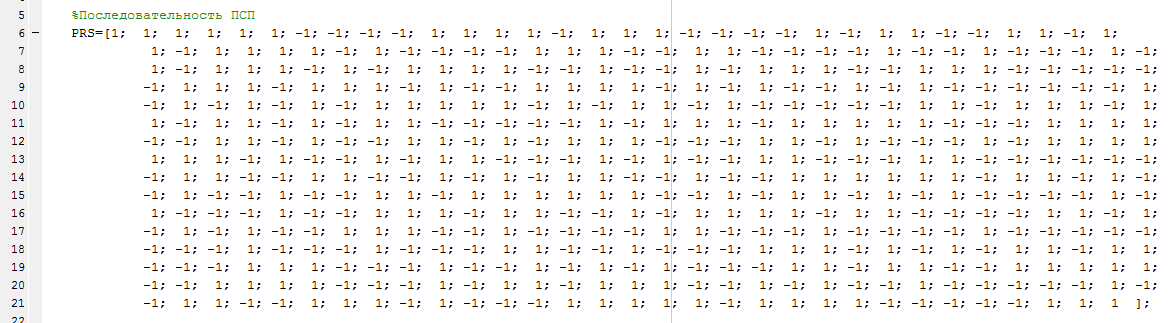
\includegraphics[width=0.95\textwidth]{psp}
\captionsetup{justification=centering,margin=1.0 cm}
\caption{PSP}
\label{any}
\end{figure}

Зададим последовательность перемежения:

\begin{figure}[H]
\centering
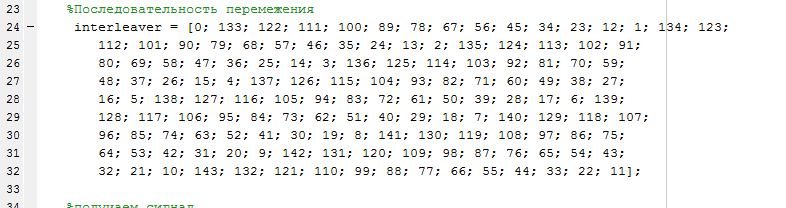
\includegraphics[width=0.95\textwidth]{interleaver}
\captionsetup{justification=centering,margin=1.0 cm}
\caption{interleaver}
\label{any}
\end{figure}

Считаем сгенерированный выходной сигнал из файла test.sig:

\begin{figure}[H]
\centering
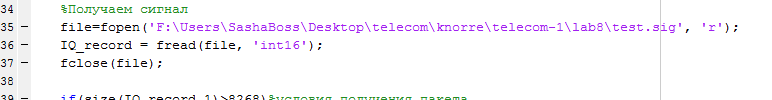
\includegraphics[width=0.95\textwidth]{read}
\captionsetup{justification=centering,margin=1.0 cm}
\caption{Reading signal}
\label{any}
\end{figure}

Согласно заданию выделяем реальную и мнимую части сигнала:

\begin{figure}[H]
\centering
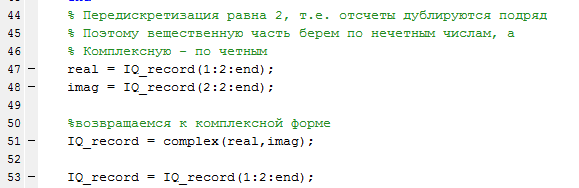
\includegraphics[width=0.95\textwidth]{reim}
\captionsetup{justification=centering,margin=1.0cm}
\caption{Real and imaginary parts}
\label{sig}
\end{figure}

Демодулируем и строим матрицу Уолша:

\begin{figure}[H]
\centering
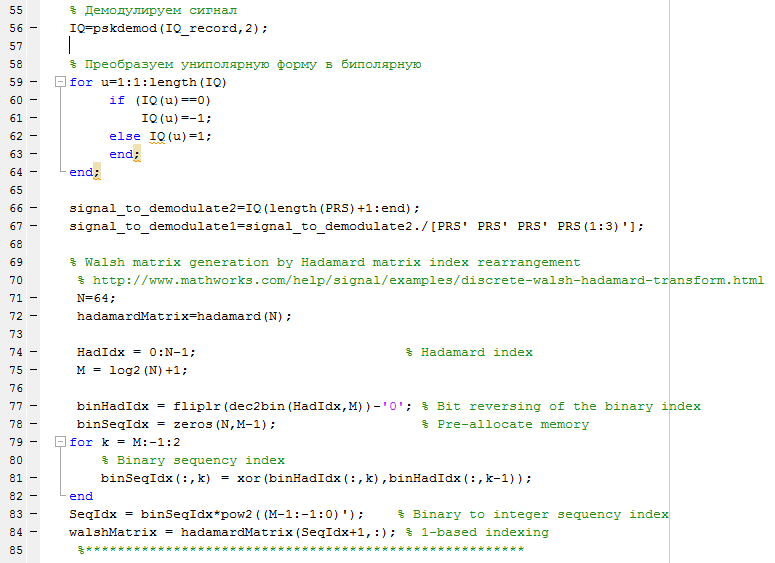
\includegraphics[width=0.95\textwidth]{walsh}
\captionsetup{justification=centering,margin=1.0cm}
\caption{Walsh matrix computation}
\label{sig}
\end{figure}

Переходим к двоичному виду:

\begin{figure}[H]
\centering
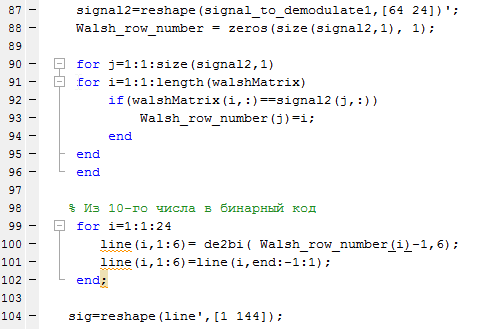
\includegraphics[width=0.95\textwidth]{preint}
\captionsetup{justification=centering,margin=1.0cm}
\caption{Conversion to binary}
\label{sig}
\end{figure}

Производим декодирование с учётом перемежения:

\begin{figure}[H]
\centering
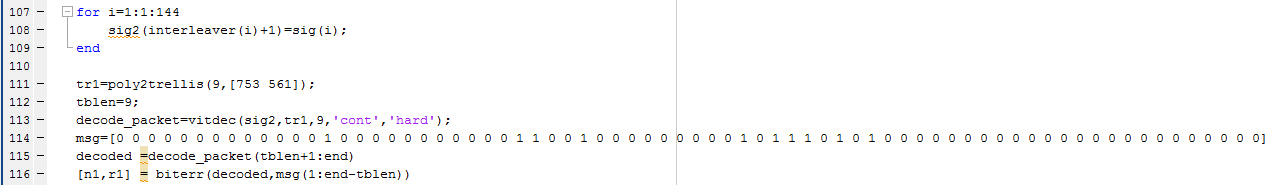
\includegraphics[width=0.95\textwidth]{postint}
\captionsetup{justification=centering,margin=1.0cm}
\caption{Decoding}
\label{sig}
\end{figure}

Отсутствие ошибок в декодированном пакете сигнализирует о верном решении задачи.

\vspace{8cm}

\section{Выводы.}

В данной работе мы создали модель приемника, выполняющую операции демодуляции, деперемежения и декодирования. Единичный опыт показал пригодность данной модели.


\end{document}
